\chapter{Protein-GAG binding site prediction via electrostatic potential analysis}

In this chapter we present a simple and yet efficient method for predicting
where on a protein a GAG would most likely bind, suggesting which amino acid
residues are likely to be involved in the interaction and which are not. The
method is based on numerical simulation of the electrostatic (i.e.\ Coulomb)
potential of the protein in water solution, and manual evaluation of the
topology of the Coulomb potential in space. Subsequently, we apply that method
to IL-10 and report our findings.

\section{Motivation}
\label{bspred:motivation}

Classical molecular docking approaches are used for creating binding predictions
for a given receptor-ligand system. Primarily, the correctness of a prediction
depends on the quality of the underlying physical or phenomenological model, and
whether the system under investigation is within the scope of validity of the
model. Since most molecular docking methods are trained for analyzing a limited
Cartesian volume in a \textit{local} search, application to larger search spaces
such as in \textit{global} docking dramatically lowers the confidence in the
resulting prediction. Therefore, common molecular docking methods should be
applied locally, and hence require \textit{a priori} knowledge about where on
the receptor the ligand most likely binds. The decision where to center the
local search on should be based on reliable data, otherwise the docking study
might be pointless. In the best case, knowledge about the binding region (the
region on the receptor that the ligand binds to) comes from experimental data,
e.g.\ from mutagenesis or NMR studies. However, in many cases no such
experimental data is available, as is unfortunately true for the IL-10-GAG
system. In such situations, it makes sense to consider \textit{in silico}
methods for prediction the binding region.

With respect to protein-GAG systems, there is only few published work on this
topic. In \cite{hp_binding_sites_mulloy_2006}, Forster and Mulloy used AutoDock
version 2.4 \cite{autodock24} for globally docking rigid heparin molecules to
antithrombin and FGF2, and found that their docking procedure gave good
agreement with the corresponding crystal structures regarding the overall
position of the heparin binding sites. The authors state that the method may be
used as \enquote{hypothesis generation tool} rather than for providing
\enquote{details of interactions between specific atoms}. In another work
\cite{gandhi_bmp_heparin_binding_sites_2012}, the authors used PatchDock
\cite{patchdock_2002} for globally docking rigid heparin oligosaccharides to
BMP-2 and BMP-14 and state that \enquote{while there has been no validation of
the accuracy of the PatchDock scoring function for heparin interactions, these
docking results suggest the presence of two GAG binding sites in BMP-2}. In
\cite{rogers_gag_prot_prot_2011}, the authors used a mixture of two docking
softwares for rigid-body docking of GAG structures \enquote{to the entire
molecular surface of the protein to locate the most favorable binding sites}.
Also in \cite{bitomsky_gag_docking_1999}, the authors report success in
predicting heparin binding sites on proteins using various docking methods.

The above-cited studies do by no means provide a complete picture, but obviously
some of the established docking methods seem to be able to reflect certain
properties of protein-GAG systems. This is remarkable since none of these
docking methods has been specifically optimized for GAG ligands, let alone for
global docking, and strictly spoken, when applied to protein-GAG systems, these
docking methods are applied outside their scope of validity. We postulate that
the reason for the surprising success in named studies is that protein-GAG
complexes are strongly driven by Coulomb interaction and that mentioned docking
methods incorporate Coulomb interaction with a significant weight in their
scoring functions.

In fact, heparin has the highest negative charge density among biological
macromolecules \cite{capila_linhardt_hep_prot_2002}. Standard literature on
protein-GAG systems such as
\cite{essentials_glycobiology_gags_2009,gandhi_structure_2008} stresses the
role of charge-charge interaction in protein-GAG systems in general. Many
publications focusing on individual protein-GAG systems identify charge
complementary as one of the driving mechanisms of the interaction between GAG
and protein
\cite{gandhi_bmp_heparin_binding_sites_2012,faham_heparin_1996,%
pichert_characterization_2012,rogers_gag_prot_prot_2011}.

We can conclude that the importance of Coulomb interaction is a distinctive
feature of protein-GAG systems. Notably, compared to other molecular interaction
types, the Coulomb interaction is a long range interaction and therefore
dominates all other contributions for larger distances. As of these
considerations, it seems to be reasonable to perform protein-GAG binding region
prediction purely based on the strength and topology (i.e.\ the
shape/distribution) of the electrostatic potential in the volume surrounding the
protein.

For a set of reference systems, we have investigated the relation between the
strength and topology of Coulomb potential and the actual experimentally
determined GAG binding site in order to determine whether the electrostatic
properties alone can assist in predicting a receptor GAG binding region. The
result of this study, be it positive or negative, in any case further enlightens
the role of Coulomb interaction in protein-GAG systems.


\section{Method}

\subsection{Coulomb potential simulation}

For a given protein, we calculated its electrostatic potential with a
finite-difference numerical solver applied to the linearized Poisson-Boltzmann
(PB) equation. The PB equation is widely used for implementing a class of
implicit solvent models to describe solvent-mediated electrostatic interactions.
These models have been demonstrated to be reliable in reproducing the energetics
when compared with explicit solvent molecular dynamics simulations and
experimental measurements for a wide range of systems \cite{honig_estatic_1995}.
In the PB model we have applied, the solute (protein) is described by an
atomic-detail representation, while the solvent molecules are treated as a
continuum. The solute is modeled as a dielectric body whose shape is defined by
atomic coordinates and atomic radii. A set of point charges at the atomic
centers produces an electrostatic field in the solute region as well in the
solvent region. The overall electrostatic field is the sum of the Coulombic
field of the solute and the corresponding reaction field of the polarizable
solvent.

We used the PBSA program shipped with AmberTools 13 \cite{case_amber_12} with
default parameters and a finite element grid spacing of \SI{1}{\angstrom} for
calculating the overall electrostatic potential of any given protein in water.
The atomic radii and point charges of the protein were parameterized according
to the FF99SB force field \cite{case_amber_12}. After patching PBSA (and
contributing those patches back to the AmberTools project), we were able to
extract the Coulomb data from PBSA in units of
\si{\kilo\calory\per\mole\per\elementarycharge} and in a file format readable by
the visualization software VMD \cite{vmd_1996}.

\subsection{Coulomb potential evaluation}

Many authors discussing the properties of a certain GAG receptor protein depict
the electrostatic potential of the protein mapped onto its molecular surface, as
done in \cite{rogers_gag_prot_prot_2011,%
Gandhi01102009,sapay_hs_growthfactors_2011,%
gandhi_bmp_heparin_binding_sites_2012,sost_heparin_2009,%
catK_cs4_crystal_structure_2008,hydrolase_gags_2011,gandhi_structure_2008,%
imberty_gag_prot_carbres_2007,gags_as_polyelectrolytes_2010}. Most of these
works lack clear conclusions from this kind of analysis, which in our opinion is
the result of two conceptual flaws of the approach. First of all, by only
looking at the surface one ignores the properties of the potential in the volume
surrounding the protein, i.e.\ one misses to analyze the potential which a GAG
feels when it is in the neighborhood of a protein, and one especially misses to
see how a GAG may be guided by a certain topology of the potential in space.
Secondly, an unfortunately often overseen disadvantage of the surface-mapping
approach is that the PB approximation of the electrostatic potential is
\text{most} error-prone near the dielectric boundary, i.e.\ right on the
molecular surface. In \cite{estatic_proteins_warshel_2006}, Warshel et al.\
write that \enquote{the problem is not the well-known bulk contribution from the
surroundings [\dots], but the polarization at the microscopic boundaries of the
simulation spheres}.

The data we obtain from PBSA are the values of the electrostatic potential on
the grid centers of a three-dimensional grid, spanning a volume of a certain
size including the protein as well as its surroundings. In contrast to what is
usually done, we decided to analyze the properties of the electrostatic
potential within the entire protein-surrounding volume, \textit{i)} for working
around the uncertainty of the data near the boundary, and \textit{ii)} for
looking at the complete picture.

We therefore analyzed the topology and strength of the potential with an
isosurface representation while varying the isosurface value. This procedure,
which will become more clear in \cref{bspred:appl_discussion} below, allows for
understanding the distribution of the potential in space as well as how strongly
it would affect a ligand. A characteristic isovalue was determined individually
for each protein for the case where only a small part of the isosurface is
protruding into space further than the molecular surface of the receptor. This
characteristic isovalue may provide an idea about the strength of the
electrostatic interaction between ligand and receptor in the bound state. The
isosurface visualization was performed using VMD \cite{vmd_1996}.


\section{Application to reference systems}
\label{bspred:application}

We have analyzed the electrostatic potential of the following experimentally
characterized and well-understood protein-GAG systems: basic fibroblast growth
factor (FGF2) in complex with a heparin (HP) tetrasaccharide, PDB ID 1BFB,
\SI{1.9}{\angstrom} resolution; the CD44 hyaluronic acid binding domain in
complex with a hyaluronan heptasaccharide (HA), PDB ID 2JCQ,
\SI{1.3}{\angstrom}; and stromal cell-derived factor-1 (SDF-1) in complex with a
HP disaccharide, PDB ID 2NWG, \SI{2.1}{\angstrom}.

% TODO: include this? Compared to effort, I dont see the value.
%Furthermore, we have applied the electrostatic potential analysis to Sclerostin
%(SOST), whose interaction with heparin has recently been investigated via NMR
%\cite{sost_heparin_2009}.


\subsection{Results and discussion}
\label{bspred:appl_discussion}

\subsubsection{FGF2}

\begin{figure}
\centering
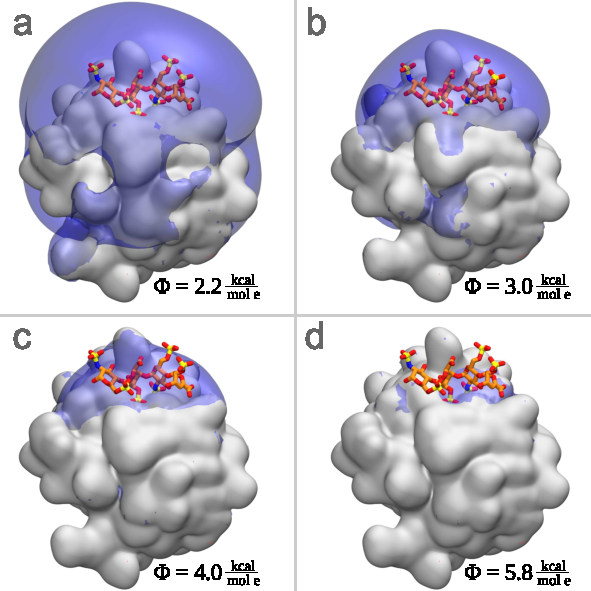
\includegraphics[width=0.9\textwidth]{gfx/bspred/fgf2_coulomb_isosurfaces_different_values_03_ds.pdf}
\caption[]{
Isosurface representation of FGF2's Coulomb potential (blue), shown for four
different isovalues isovalues $\Phi$, in increasing order. The molecular surface
of FGF2 is shown in gray, its heparin ligand pose as determined experimentally
is shown as sticks with carbon atoms in orange (structure taken from PDB ID
1BFB).}
\label{fig:bspred:fgf2_multi_iso}
\end{figure}

\Cref{fig:bspred:fgf2_multi_iso} depicts the process of visualizing the
electrostatic potential of FGF2 with an isosurface representation and varying
isovalue. The four isovalues shown are positive ones, and the isosurfaces
therefore represent \textit{attraction} for GAGs. Isosurfaces for isovalues of
comparable absolute value and opposite sign are \enquote{within} the molecular
surface, i.e.\ electrostatic GAG \textit{repulsion} is negligible in case of
FGF2.

\Cref{fig:bspred:fgf2_multi_iso}a shows the isosurface corresponding to the
smallest of the four isovalues with
\SI{2.2}{\kilo\calory\per\mole\per\elementarycharge}. This is still a strong
potential, yielding significant potential energies for charged ligand molecules:
\SI{2.2}{\kilo\calory\per\mole} is almost four times larger than the thermal
energy at \SI{300}{\kelvin}. From this representation we learn that FGF2 is
highly polar on its global scale: in the depicted top direction, the isosurface
protrudes into space far beyond the molecular surface, whereas it does not
surpass the molecular surface at the bottom. We conclude that FGF2 may interact
with GAGs over large distances (several times larger than what can be
considered a molecular contact), and with a clear preference towards one side
of the protein (the top side in the orientation as shown in
\cref{fig:bspred:fgf2_multi_iso}). Furthermore, we observe that the
experimentally determined natural heparin ligand pose is bound to that side of
FGF2.

Panels a, b, and c of \cref{fig:bspred:fgf2_multi_iso} visualize the process of
increasing the isovalue while observing the response of the isosurface. This
process serves two purposes. Firstly, the shape change of the isosurface with
increasing isovalue provides insight about the direction into which a negatively
charged molecule would be \textit{guided} by the Coulomb potential once caught
(the gradient of the potential). Secondly, it allows for further narrowing down
those regions in space near the molecular surface of FGF2 where electrostatic
attraction is strongest, because the surface protrudes less and less into space
with increasing isovalue. Regarding directionality, the isosurface clearly
contracts itself towards a certain region on FGF2's surface, considering panels
a, b, and c of \cref{fig:bspred:fgf2_multi_iso}. It is that region where we also
find the experimentally determined ligand pose. In panel c we observe that there
is only a small region in space outside of FGF2 where the Coulomb potential is
as large as
\SI{4.0}{\kilo\calory\per\mole\per\elementarycharge}, which is about seven times
stronger than the thermal energy at room temperature, considering a single test
charge. With an electrostatic attraction as strong as this and clearly no other
regions near the molecular surface of FGF2 with a comparably strong Coulomb
potential, it is unlikely that a negatively charged ligand molecule tends to
interact anywhere else with FGF2 than in that region.

\Cref{fig:bspred:fgf2_multi_iso}d shows the isosurface for what we call the
\textit{characteristic} isovalue, which (roughly) is that isovalue for which
only a residual part of the isosurface is protruding into space further than the
molecular surface of the receptor protein. The goal of this representation is to
scan the direct vicinity of the molecular surface of the protein for the regions
of strongest electrostatic attraction, and to be able to quantify that
attraction. In case of FGF2, we found that value to be about
\SI{6}{\kilo\calory\per\mole\per\elementarycharge}, which is about 10 times
larger than the thermal energy. While the isosurface representation in panel c
localizes the region of interest within a volume still larger than the size of
the heparin ligand, the isosurface in panel d narrows it further down to one
major \enquote{hot spot}. We observe a match between the position of this hot
spot and the position of those two sulfate groups of the heparin ligand that are
the main anchors of the interaction between FGF2 and heparin
\cite{faham_heparin_1996}, which is quite a remarkable result. Overall, the
topology of FGF2's electrostatic potential \textit{unambiguously} suggests
\textit{one} site for potential GAG interaction, and that site very well matches
the measured one.


\subsubsection{SDF-1}

\begin{figure}
\centering
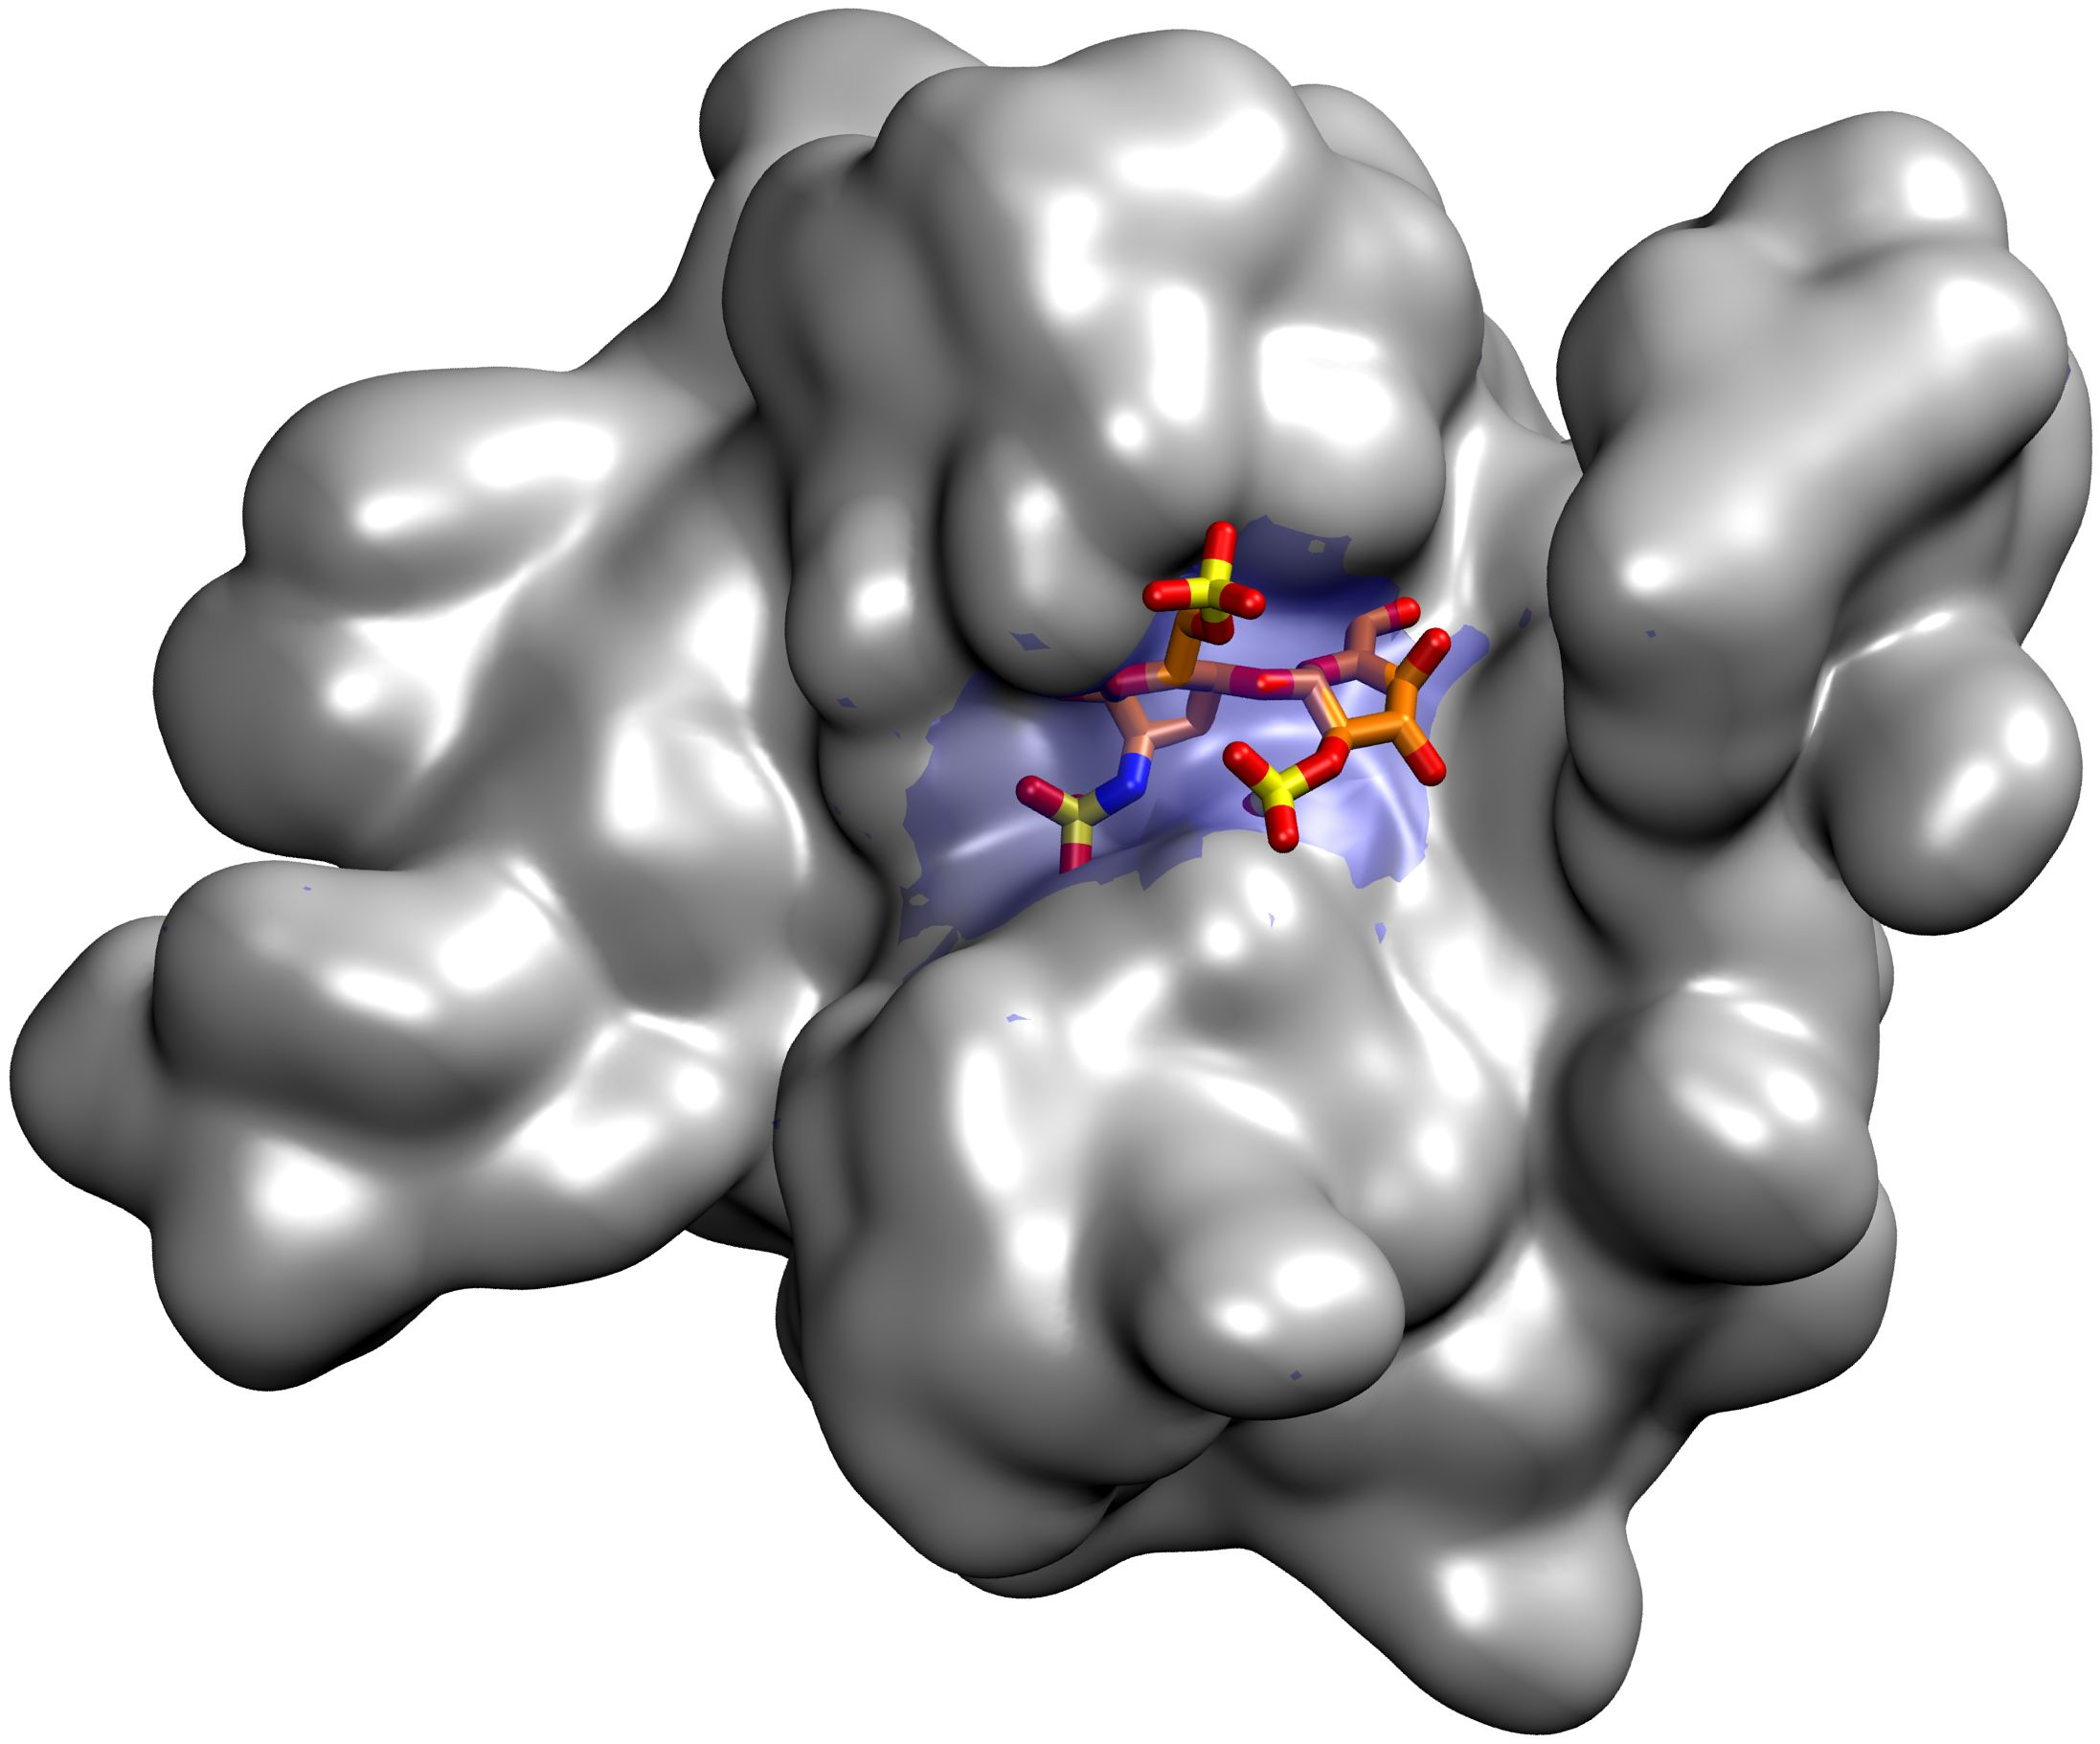
\includegraphics[width=0.7\textwidth]{gfx/bspred/sdf1_isopot_8_5_view1_rotated_jcc_pub_001.jpg}
\caption[]{
Isosurface representation of SDF-1's Coulomb potential with the characteristic
isovalue of $\Phi=\SI{8.5}{\kilo\calory\per\mole\per\elementarycharge}$ (blue).
The molecular surface of the SDF-1 dimer is shown in gray, the heparin ligand as
determined experimentally is shown in stick representation with carbon atoms in
orange (structure taken from PDB ID 2NWG).}
\label{fig:bspred:sdf1_estatic}
\end{figure}

\Cref{fig:bspred:sdf1_estatic} shows the isosurface of SDF-1's Coulomb potential
corresponding to its characteristic isovalue
$\Phi=\SI{8.5}{\kilo\calory\per\mole\per\elementarycharge}$. We see that the
ligand pose matches the region of strongest electrostatic attraction. Another
important observation is that the characteristic isovalue is significantly
larger than in case of FGF2, meaning that the electrostatic attraction of SDF-1
in the indicated region is once again stronger. In fact, SDF-1 displays the
largest characteristic isovalue we have come across during the analysis of
various different protein-GAG systems. The spatial arrangement of positively
charged residues in the shape of a cleft produces an environment in which the
attractive potential from the two sides of the cleft adds up in the center,
yielding a stronger electrostatic potential than possible with a one-sided
interaction only.

Variation of the isovalue and observing the corresponding response of the
isosurface, although not depicted in this case, has provided very similar
conclusions as in the case of FGF2: all indicators point towards \textit{one}
region on SDF-1 with a very strong electrostatic attraction at its core, as well
as the ability to attract a GAG molecule over long distances. As in case of
FGF2, the topology of SDF-1's electrostatic potential unambiguously suggests one
site for potential GAG interaction, and that site matches the experimentally
confirmed one.


\subsubsection{CD44 hyaluronic acid binding domain}

\begin{figure}
\centering
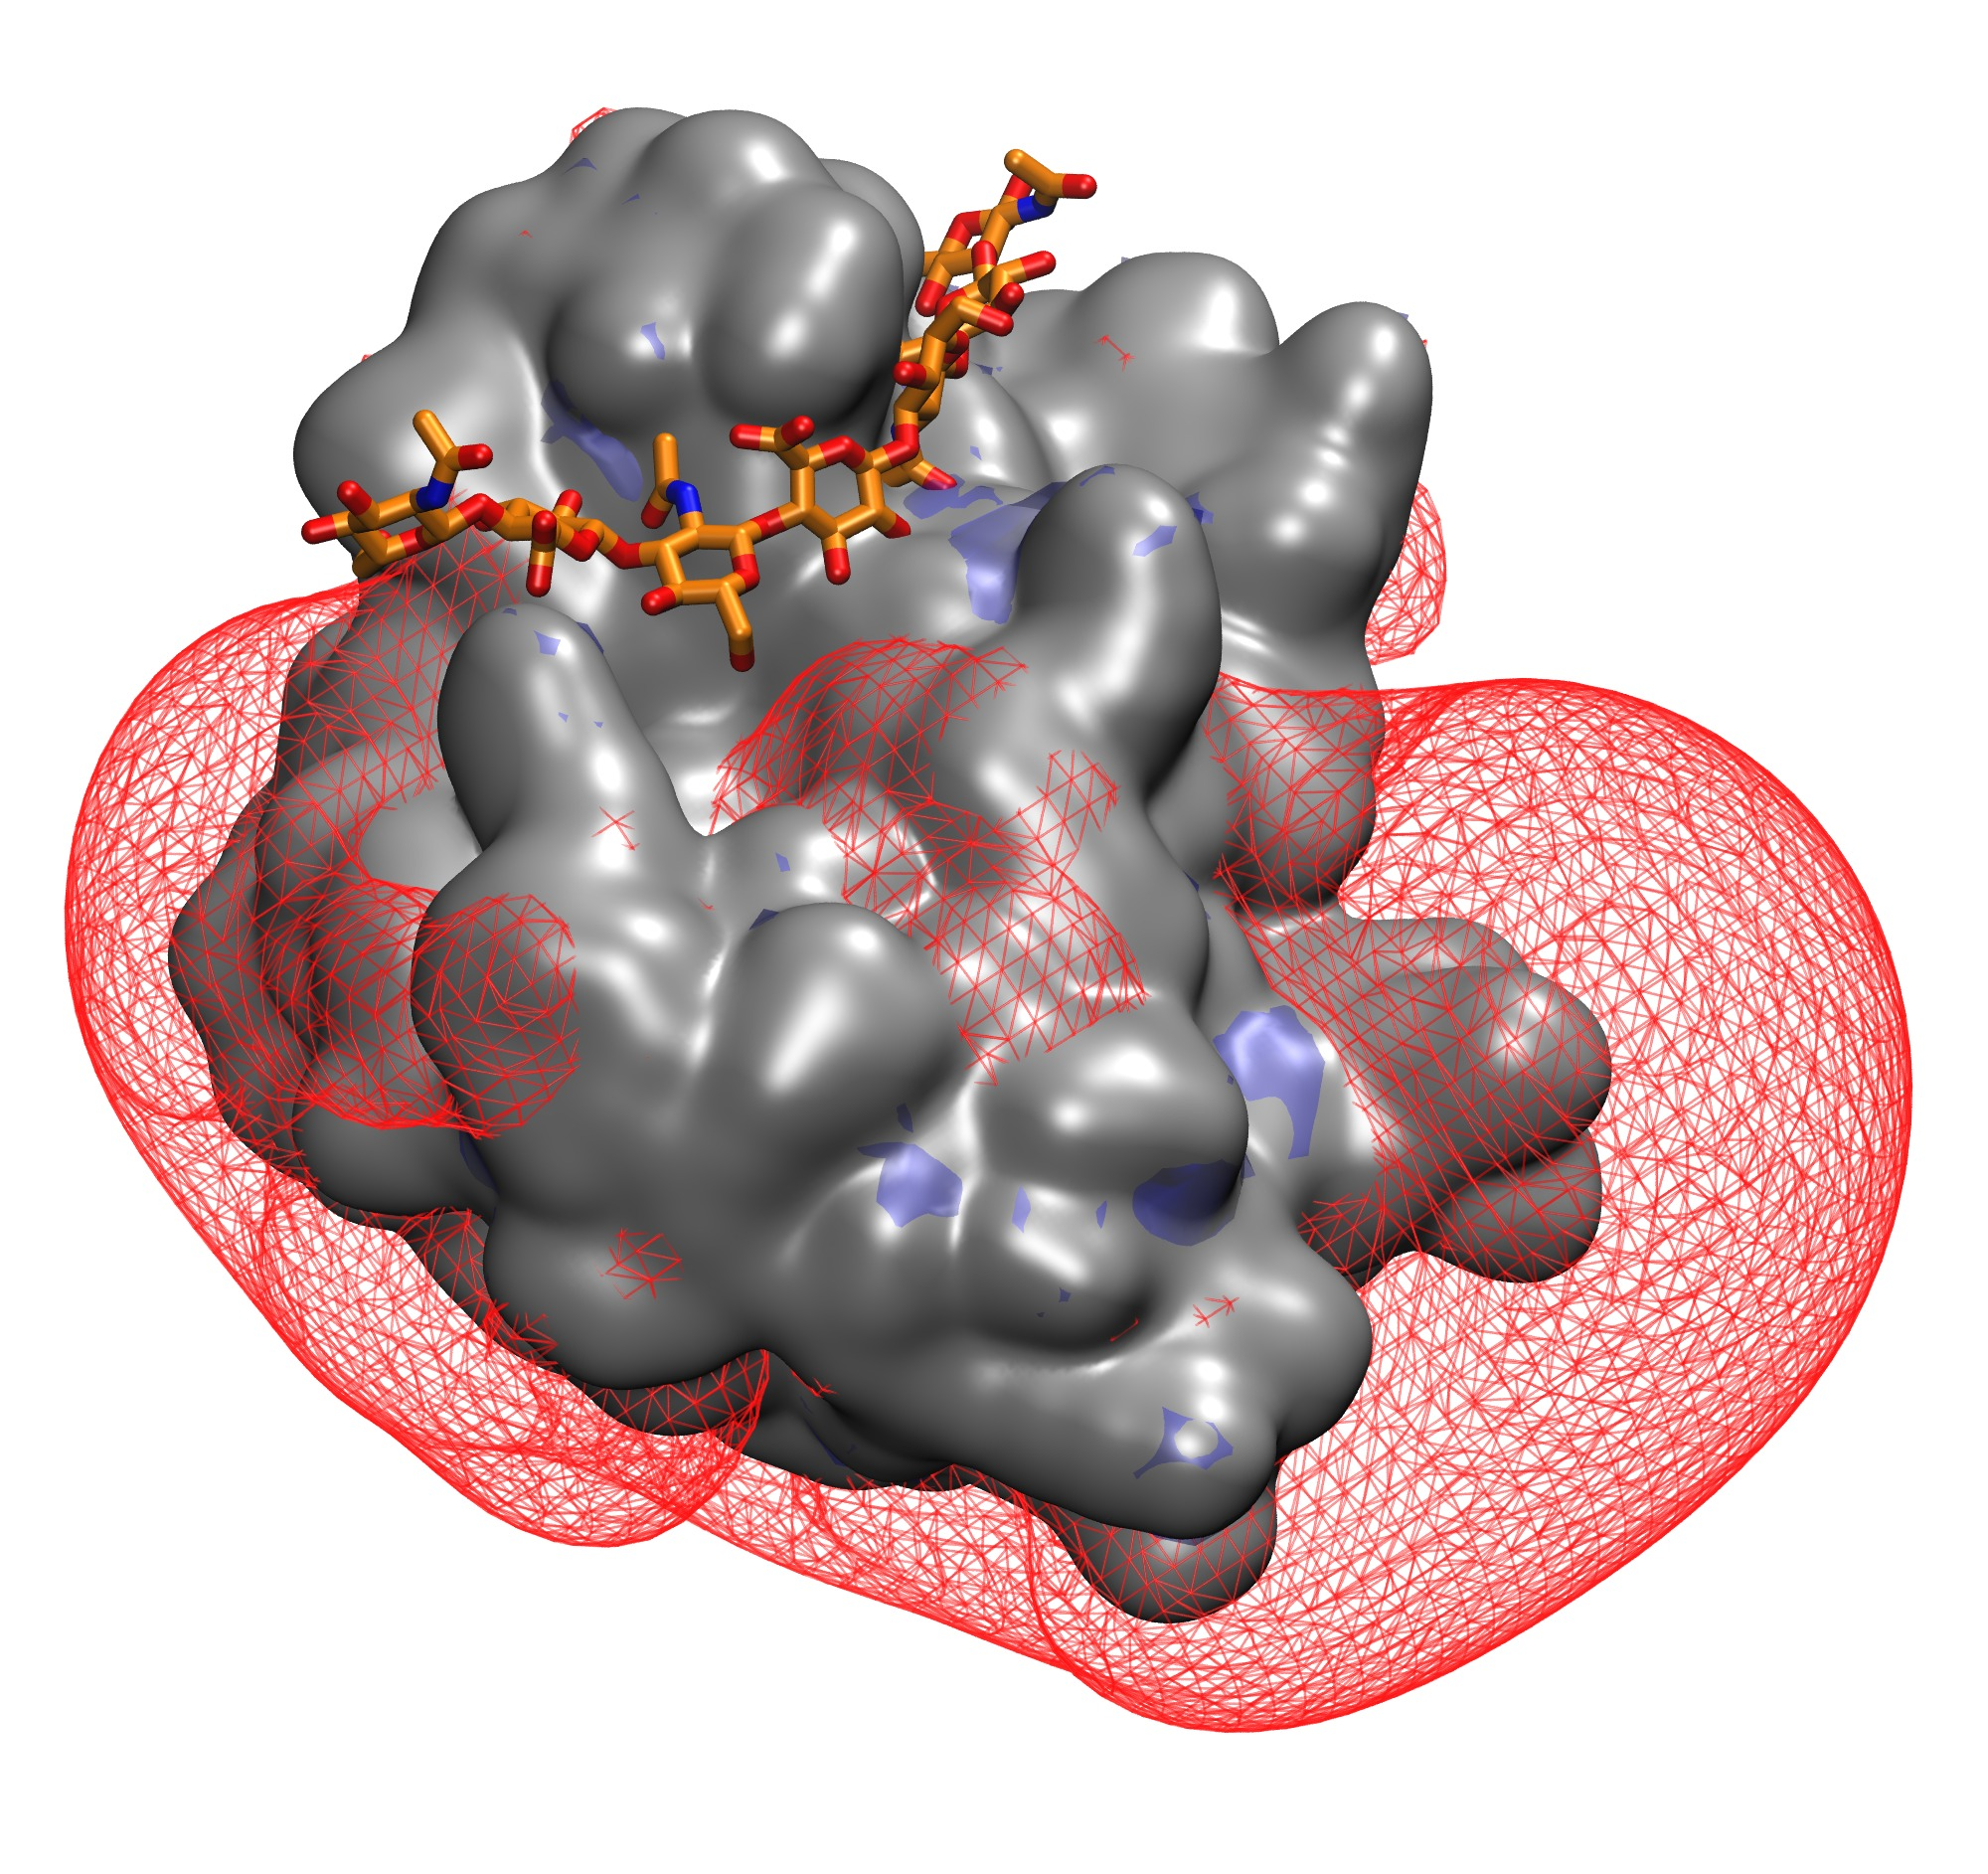
\includegraphics[width=0.7\textwidth]{gfx/bspred/2JCQ_isopot500_ligand_view1.jpg}
\caption[]{
Isosurface representation of CD44's Coulomb potential with the isovalues
$\Phi=\pm\SI{1.5}{\kilo\calory\per\mole\per\elementarycharge}$ (blue: attractive
for negative charges, red: repulsive for negative charges). The molecular
surface of the hyaluronic acid binding domain of CD44 is shown in gray, the
hyaluronan heptasaccharide ligand in the pose as determined experimentally is
shown in stick representation with carbon atoms in orange (structure taken from
PDB ID 2JCQ).}
\label{fig:bspred:cd44_estatic}
\end{figure}

CD44's interaction with hyaluronan is fundamentally different from the SDF-1-HP
and FGF2-HP systems. In \cref{fig:bspred:cd44_estatic} we see that even for the
quite small isovalue of \SI{1.5}{\kilo\calory\per\mole\per\elementarycharge}
(compared to the previously discussed systems), there is almost no (blue)
isosurface visible, meaning that the protein has no long-range electrostatic
attraction for GAGs. In direct vicinity to CD44's molecular surface some small
patches representing weak attraction for negative charges are observable.
However, their location is rather scattered. The main observation for the
CD44-HA system is that most parts of the protein have a slightly repulsive
Coulomb potential. Considering how far certain parts of the isosurface for
\SI{-1.5}{\kilo\calory\per\mole\per\elementarycharge} protrude into space, we
can conclude that the net repulsion may take effect over long distances. While
there seems to be a (weak) net repulsion for GAGs, there also is larger region
on the protein surface which appears to be rather neutral from the electrostatic
point of view, with neither of both isosurfaces piercing through the molecular
surface of CD44. It is that region where hyaluronan was shown to bind to CD44
(see \cref{fig:bspred:cd44_estatic}).

For the CD44-HA system, the main conclusion is that analysis of the
electrostatic potential fits the binding pose obtained experimentally in the
sense that there is \textit{no contradiction}. When taking a close look, the
experimentally obtained binding site contains most of the scattered patches
representing attraction for negative charges mentioned above. Furthermore, it
makes sense that the hyaluronan does not bind in one of those regions that have
been identified as being explicitly repulsive for negative charges. However,
purely based on the electrostatic potential data we would not have been able to
pinpoint a certain site as being particularly likely to attract GAGs. The major
reason for being unable to narrow down a site is that we are missing a distinct
region of significant electrostatic attraction. Accordingly, the authors of
\cite{cd44_hya_2007} point out that CD44-HA system is  \enquote{dominated by
hydrogen bonds and van der Waals forces rather than electrostatic interactions},
a quite special characteristic among protein-GAG systems.



\subsection{Conclusions}

When describing the concepts of protein-GAG interaction in all generality,
Coulomb interaction is one of the major determinants. Therefore, we claim that
evaluation of the Coulomb potential of a protein receptor alone is a systematic
and simple approach for predicting where on a protein a GAG would bind ---
\textit{if} it binds. This is an important distinction from predicting whether a
protein binds GAGs or not, which Coulomb potential analysis alone can surely
\textit{not} do reliably.

We could conclude that the presented method is very well able to make valid
predictions regarding protein-GAG binding regions. However, the most important
aspect to discuss when predicting the behavior of a system is the
\textit{certainty} of the prediction. The huge advantage of the method we have
presented here seems to be that it \textit{intrinsically} provides a good
estimate about the certainty of its own prediction. Especially, this method is
unlikely to generate false-positives. For example, the data about CD44 shown
above would have led us to state nothing more definite than \enquote{we can not
tell where a GAG would bind, however it will most likely not bind in the
repulsive regions}. At the same time the data regarding FGF2 and SDF-2 provide
undeniable support that GAGs bind where the Coulomb potential points towards,
especially regarding the large characteristic electrostatic potential isovalues
in proximity of the molecular surface. The main conclusion is that if we observe
a \textit{distinct} region of \textit{significant} electrostatic attraction,
then this is the place where a GAG would most likely bind. If the electrostatic
potential topology is as unambiguous as in case of SDF-1 or FGF2, a GAG binding
site prediction based on the presented procedure is reliable.

According to recent literature in the field (see \cref{bspred:motivation}),
global docking methods are often (mis)used for protein-GAG binding site
prediction, because no other tool seems to be established for that task. With
the presented method we seek to provide such a tool. Hence, the presented method
is in direct competition with (global) docking methods. Compared to those,
Coulomb potential evaluation is significantly less complex: it is a bare-bones
approach based on a simple physical model, whereas a docking method usually
applies a combination of both, a more complex physical and phenomenological
model. The certainty of a docking prediction is difficult to assess if the
docking method is applied outside of its scope of validity, i.e.\ to different
systems and e.g.\ search space sizes than it has been optimized for. A reason
for this is the complexity of a docking method, as of which we can not
systematically understand the behavior of the method if we leave its scope of
validity. Strictly spoken, in that case the certainty is \textit{not}
assessable, neither quantitatively nor qualitatively. Therefore, the risk for
producing false-positive predictions is much higher than in case of the method
presented by us. Here, we see a clear conceptual advantage of the Coulomb
potential evaluation over more complex methods such as global docking.

Another advantage of the proposed visualization of the electrostatic potential
via isosurface representation is that it enables the researcher to quickly grasp
the global electrostatic properties of any given protein, much better than it is
possible via mapping the potential to the molecular surface only. For instance,
this can be helpful for identifying repulsive regions in space to \textit{a
priori} exclude large regions of the protein as potential ligand binding
regions.

While the method presented here can in all generality not be used for predicting
whether a certain binding mode would be \textit{specific} or not, it can provide
insights about the binding \textit{affinity} of a certain protein-GAG system,
via evaluation of the characteristic isovalue. At the very least, this value
allows for ranking different systems, which is how we came to the conclusion
that SDF-1 has the strongest electrostatic attraction to its GAG ligand among
all protein-GAG systems we have looked at in the course of our studies.

In the motivational part we stated that the result of this study further
enlightens the role of Coulomb interaction in protein-GAG systems. Indeed, we
did not expect that the Coulomb potential topology might yield such precise
clues about the binding site as we have seen in case of FGF2 and SDF-1. This
underlines the role of Coulomb interaction in protein-GAG systems as the primary
determinant. However, we have also learned that in special cases a strong
electrostatic attraction is not required for GAG binding, as vividly shown for
the CD44-HA example.

%If we had to name a spatial resolution that would quantify the degree of detail
%the electrostatic potential analysis allows

%Besides a qualitative statements about a binding region,
% The data itself tells us when we should not perform a precise prediction.


\section{Application to IL-10}

Regarding IL-10, the shape of the potential in space provides strong evidence
that if GAGs bind to it, then most likely in a well-defined region. What makes
this prediction less certain as e.g.\ in case of SDF-1 and FGF2 is the fact that
the characteristic isovalue of the Coulomb potential in the predicted regions is
significantly smaller than in named reference systems. So far, we have no
experience whether there is a certain threshold in this value, below which we
can or should not use our prediction method anymore for deriving reliable
predictions. The low value in any case suggests that IL-10-GAG binding occurs
with lower binding affinity as is the case of  SDF-1 and FGF2 .

\begin{figure}
\centering
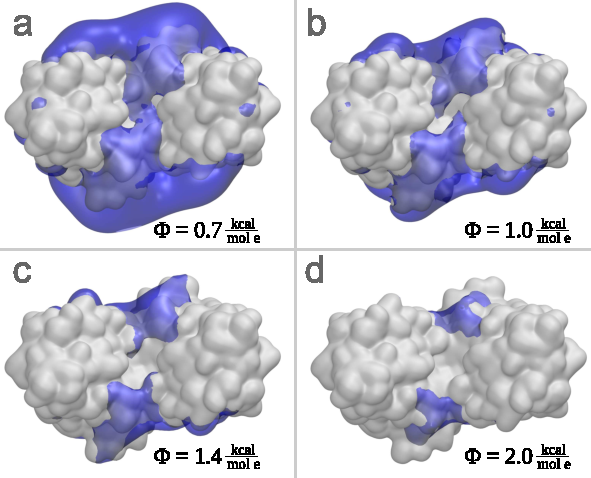
\includegraphics[width=1.0\textwidth]{gfx/bspred/il10_top_coulomb_isosurfaces_different_values_03_ds.pdf}
\caption[]{
Isosurface representation of IL-10's Coulomb potential (blue), shown for
multiple isovalues isovalues $\Phi$. The molecular surface of the IL-10 dimer is
shown in gray (structure taken from PDB ID 2ILK).
}
\label{fig:bspred:il10_multi_iso}
\end{figure}


\begin{figure}
\centering
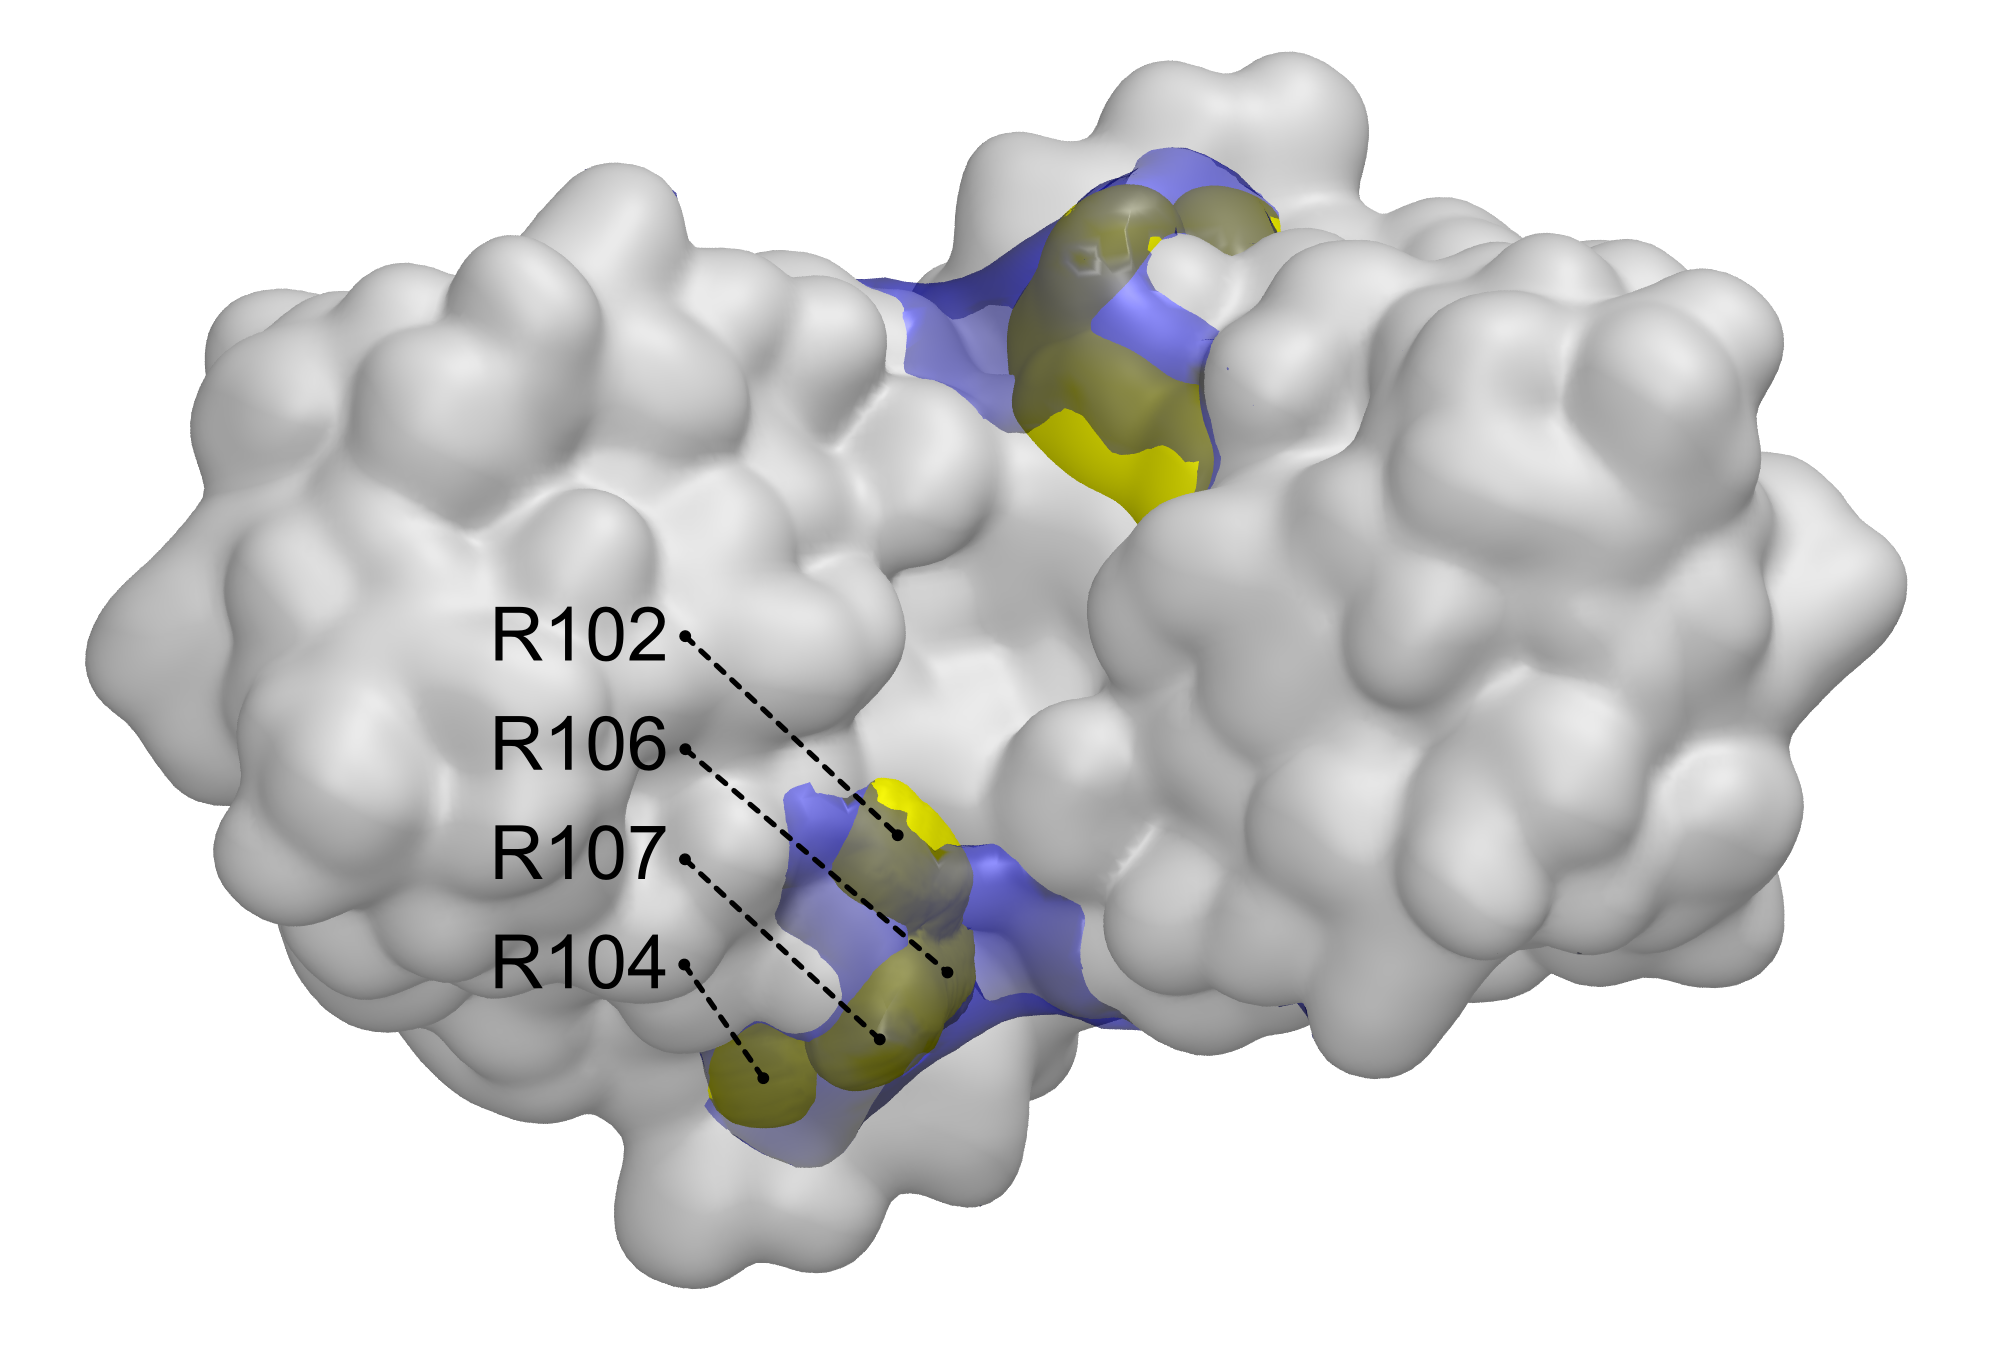
\includegraphics[width=0.9\textwidth]{gfx/bspred/SI_figure_IL-10_coulomb_isosurface_1_9kcalmol.png}
\caption[]{
Isosurface representation of IL-10's Coulomb potential with the isovalue $\Phi =
\SI{1.9}{\kilo\calory\per\mole\per\elementarycharge}$ (blue). The molecular
surface of the IL-10 dimer is shown in gray, the molecular surface of arginines
102, 104, 106, 107 is shown in yellow (structure taken from PDB ID 2ILK). This
representation allows to see where the Coulomb potential (for a given isovalue)
protrudes into space further than the molecular surface, and has been shown to
provide useful evidence about where GAGs bind to a protein \hl{(REF)}. Hence,
IL-10-GAG interaction most likely takes place within the two symmetrically
arranged regions indicated here.
}
\label{fig:bspred:il10_estatic_pred}
\end{figure}


\subsection{Results and discussion}
\hl{INCORPORATE:} The method surely is more useful than the popular method of
heparin binding site consensus sequence search (cardin, weintraub) (hileman,
linhardt), which has already been applied to interleukin-10 before. Its about
structure, not sequence, that is also why Forster and Mulloy state that
\enquote{though some 'consensus sequences' for heparin binding have been
identified, they are neither necessary nor sufficient to define a heparin
binding site} \cite{hp_binding_sites_mulloy_2006}.



\hl{Generalize this section, keep details for DMD chapter. At the moment most of
this is simply copied from the DMD manuscript.}
The electrostatic potential often dominates protein-GAG interaction
\cite{gandhi_structure_2008}. In this section, we discuss the electrostatic
properties of the receptors in the TDS with the goal to determine how these
properties could assist defining a receptor target region for DMD and also to be
able to relate docking performance to electrostatic characteristics of the
receptor.


\hl{put the following back in DMD part?}
Furthermore, this analysis shows that knowledge
about the electrostatic potential distribution in space can be used to choose a
reasonable ligand \enquote{entry lane} orientation for the tMD pulling process.


\subsection{Conclusions}
Short conclusional text regarding IL-10 GAG binding prediction.